%!TEX root = restart.tex
\section{Adjoint based flow optimization\label{sec:Adjoint-method}}


\subsection{Optimal control problem formulation\label{par:Optimization-Problem}}

In addition to our governing equations $\sys\left(\state,\control\right)=0$,
we also introduce a cost function $\cost$, which we assume to be
in $C^{2}$:

\begin{eqnarray*}
	\cost: & \mathbb{R}^{\nlinks T}\times\mathbb{R}^{\ncontrols T} & \rightarrow\mathbb{R}\\
	& \left(\state,\control\right) & \mapsto\cost\left(\state,\control\right)
\end{eqnarray*}
which returns a scalar that serves as a metric of performance of the
state and control values of the system. We wish to minimize the quantity
$\cost$ over the set of control parameters $\control$, while constraining
the state of the system to satisfy the governing equations $\sys\left(\state,\control\right)=0$,
which is, again, the concatenated version of~\eqref{eq:main-ge} or~\eqref{eq:syseq-god}.
We summarize this with the following optimization problem:

\begin{eqnarray}
	\underset{\control}{\min} & \cost\left(\state,\control\right)\nonumber \\
	\text{subject to:} & \sys\left(\state,\control\right)=0\label{eq:op-problem}
\end{eqnarray}
Both the cost function and governing equations may be non-convex in
this problem.


\subsection{Calculating the gradient\label{par:Calculating-the-gradient}}

We wish to use gradient information in order to find control values
$\control^{*}$ that give locally optimal costs $\cost^{*}=\cost\left(\state\left(\control^{*}\right),\control^{*}\right)$.
Since there may exist many local minima for this optimization problem~\eqref{eq:op-problem}
(which is non-convex in general), gradient\emph{ }methods do not guarantee
global optimality of $\control^{*}$\emph{. }Still, nonlinear optimization
methods such as interior point optimization utilize gradient information
to improve performance~\cite{Andreas2005}.

In a descent algorithm, the optimization procedure will have to descend
a cost function, by coupling the gradient, which, at a nominal point
$\left(\nominal{\state},\nominal{\control}\right)$ is given by:

\begin{equation}
	d_{\control}\cost\left(\nominal{\state},\nominal{\control}\right)=\evaluate{\pfrac{\cost\text{\ensuremath{\left(\state,\control\right)}}}{\state}}{\nominal{\state},\nominal{\control}}\Dfrac{\state}{\control}+\evaluate{\pfrac{\cost\text{\ensuremath{\left(\state,\control\right)}}}{\control}}{\nominal{\state},\nominal{\control}}\label{eq:j-v}.
\end{equation}


The main difficulty is to compute the term $\Dfrac{\state}{\control}$.
Next we take advantage of the fact that the derivative of $H\left(\state,\control\right)$
with respect to $\control$ is equal to zero along trajectories of
the system:

\begin{equation}
	d_{\control}\sys\left(\nominal{\state},\nominal{\control}\right)=\evaluate{\pfrac{\sys\text{\ensuremath{\left(\state,\control\right)}}}{\state}}{\nominal{\state},\nominal{\control}}\Dfrac{\state}{\control}+\evaluate{\pfrac{\sys\text{\ensuremath{\left(\state,\control\right)}}}{\control}}{\nominal{\state},\nominal{\control}}=0\label{eq:h-v}.
\end{equation}


The partial derivative terms, $\Hx\in\mathbb{R}^{\nlinks\ntime\times\nlinks\ntime}$,
$\Hu\in\mathbb{R}^{\nlinks\ntime\times\ncontrols\ntime}$, $\Jx\in\mathbb{R}^{\nlinks\ntime}$,
and $\Ju\in\mathbb{R}^{\ncontrols\ntime}$, can all be evaluated (more
details provided in Section~\ref{sub:Evaluating--and}) and then
treated as constant matrices. Thus, in order to evaluate $d_{\control}\cost\left(\nominal{\state},\nominal{\control}\right)\in\mathbb{R}^{\ncontrols\ntime}$,
we must solve a coupled system of matrix equations.
\begin{note}
	In~\eqref{eq:h-v}, $\Hx$ and $\Hu$ might not necessarily be defined,
	either because $f$ itself is not smooth (note that we took $f$ to
	be $C^{2}$ to avoid this problem), and/or because $\god$ is not
	smooth. The derivations below are valid when the partials $\Hx$ and
	$\Hu$ can indeed be taken. There are several settings in which the
	conditions for differentiability are satisfied, see in particular~\cite{Gugat2005,Flasskamp2012}.
\end{note}

\paragraph{Forward system.\label{par:Forward-system}}

If we solve for $\Dfrac{\state}{\control}\in\mathbb{R}^{\nlinks\ntime\times\ncontrols\ntime}$
in~\eqref{eq:h-v}, which we call the \emph{forward system}:

\[
	\Hx\Dfrac{\state}{\control}=-\Hu,
\]
then we can substitute the solved value for $\Dfrac{\state}{\control}$
into~\eqref{eq:j-v} to obtain the full expression for the gradient.
Section~\ref{sub:Evaluating--and} below gives details on the invertibility
of $\Hx$, guaranteeing a solution for $\Dfrac{\state}{\control}$.


\paragraph{Adjoint system.\label{par:Adjoint-system}}

Instead of evaluating $\Dfrac{\state}{\control}$ directly, the adjoint
method solves the following system, called the adjoint system,
for a new unknown variable $\lambda\in\mathbb{R}^{\nlinks\ntime}$
(called the adjoint variable):

\begin{equation}
	\Hx^{T}\lambda=-\Jx^{T}\label{eq:adjoint}
\end{equation}
Then the expression for the gradient becomes:

\begin{equation}
	d_{\control}\cost\left(\nominal{\state},\nominal{\control}\right)=\lambda^{T}\Hu+\Ju\label{eq:adjoint-grad}
\end{equation}
We define $\degree{\state}$ to be the maximum junction degree on
the network:

\begin{equation}
	\degree{\state}=\max_{\jn\in\jns}\left(\ninc_{\jn}+\nout_{\jn}\right),\label{eq:dx}
\end{equation}
and also define $\degree{\control}$ to be the maximum number of constraints
that a single control variable appears in, which is equivalent to:

\begin{equation}
	\degree{\control}=\max_{\condiscrete{}{}\in\control}\sum_{\jn\in\jns:\condiscrete{}{}\in\junccon{\jn}{\tind}}\left(\ninc_{\jn}+\nout_{\jn}\right)\label{eq:dv}.
\end{equation}


Note that $\left\{ \convar\in\junccon{\jn}{\tind}:\jn\in\jns\right\} $
is a $\tind$-dependent set. By convention, junctions are either actuated
or not, so there is no dependency on $\tind$, i.e. if $\exists\tind$
s.t. $\convar\in\junccon{\jn}{\tind}$, then $\forall\tind$, $\convar\in\junccon{\jn}{\tind}$.

Using these definitions, we show later in Section~\ref{sub:Complexity-of-solving}
how the complexity of computing the gradient is reduced from $O(\degree{\state}\nlinks\ncontrols\ntime^{2})$
to $O(\ntime\left(\degree{\state}\nlinks+\degree{\control}\ncontrols\right))$
by considering the adjoint method over the forward method.

A graphical depiction of $D_{\state}$ and $D_{\control}$ are given
in Fig.~\ref{fig:Depicting--and}
\begin{figure}
	\begin{centering}
		\subfloat[\label{fig:genneta}]{\begin{centering}
			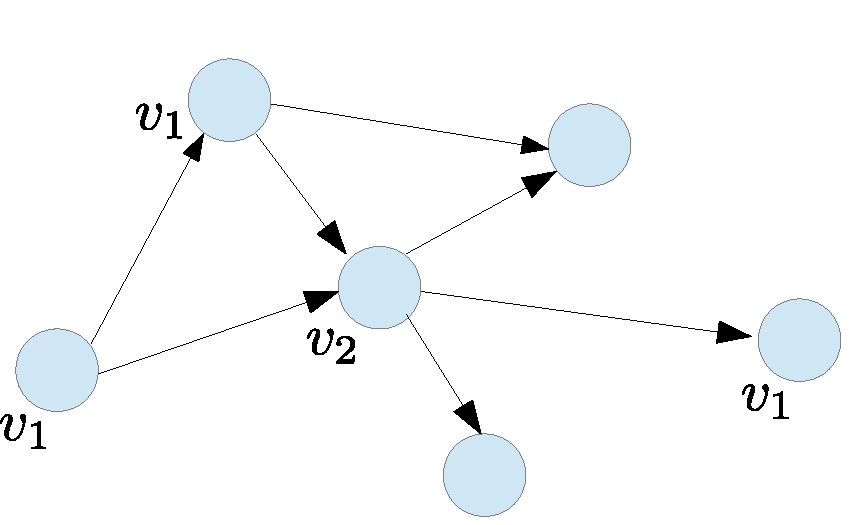
\includegraphics[width=0.33\columnwidth]{figs-gen/gen-net}
			\par\end{centering}
						
			}\subfloat[\label{fig:gennetb}]{\begin{centering}
			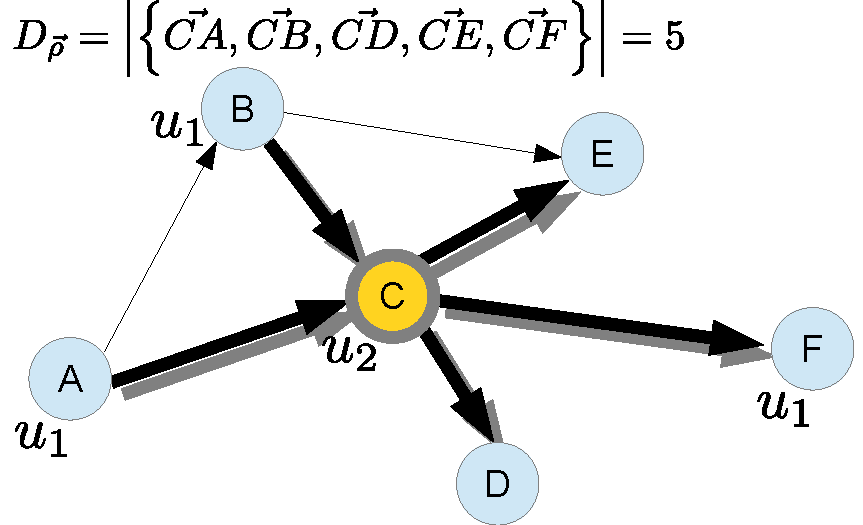
\includegraphics[width=0.33\columnwidth]{figs-gen/gen-net-dx}
			\par\end{centering}
						
			}\subfloat[\label{fig:gennetc}]{\begin{centering}
			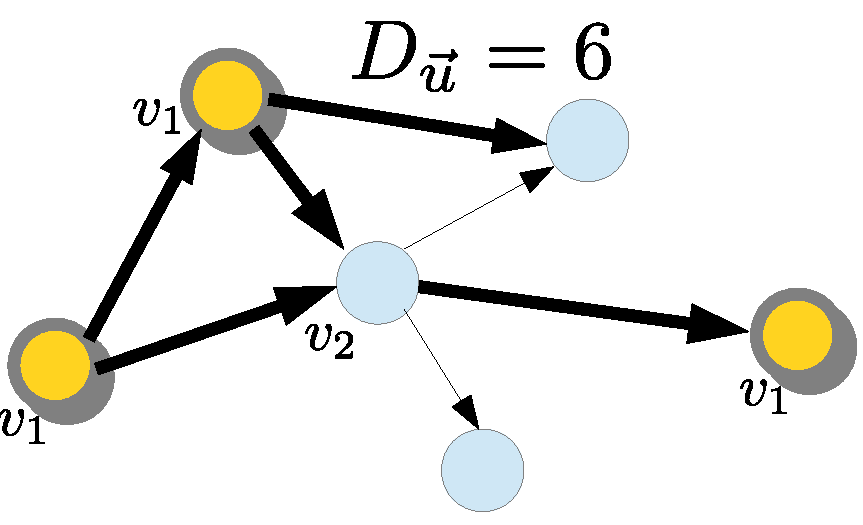
\includegraphics[width=0.33\columnwidth]{figs-gen/gen-net-dv}
			\par\end{centering}
						
		}
		\par\end{centering}
				
		\caption{Depiction of $D_{\state}$ and $D_{v}$ for an arbitrary graph. Fig.~\ref{fig:genneta}
			shows the underlying graphical structure for an arbitrary PDE network.
			Some control parameter $\convar_{1}$ has influence over junctions
			$A$, $B$, and $F$, while another control parameter $\convar_{2}$
			has influence over only junction $C$. Fig.~\ref{fig:gennetb}
			depicts the center junction having the largest number of connecting
			edges, thus giving $D_{\state}=5$. Fig.~\ref{fig:gennetc} shows
			that control parameter $\convar_{1}$ influences three junctions with
			sum of junctions degrees equal to six, which is maximal over the other
			control parameter $\convar_{2}$. leading to the result $D_{\control}=6$.
			Note that in Fig.~\ref{fig:gennetc}, the link going from junction
			$A$ to junction $B$ is counted twice: once as an outgoing link $\vec{AB}$
			and once as in incoming link $\vec{BA}$.\label{fig:Depicting--and}}
		\end{figure}
		.Freeway networks are usually considered to have topologies that are
		nearly planar, leading to junctions degrees which typically do not
		exceed 3 or 4, regardless of the total number of links. Also, from
		the locality argument for control variables in Section~(\ref{sec:State,-control,-and}),
		a single control variable's influence over state variables will not
		grow with the size of the network. Since the $\degree{\state}$ and
		$\degree{\control}$ typically do not grow with $\nlinks\ntime$ or
		$\ncontrols\ntime$ for freeway networks, the complexity of evaluating
		the gradient for such networks can be considered linear for the adjoint
		method.
				
				
		\subsection{Evaluating the partial derivatives\label{sub:Evaluating--and}}
				
		While no assumptions are made about the sparsity of the cost function
		$\cost$, the networked-structure of the PDE system and the Godunov
		discretization scheme allows us to say more about the structure and
		sparsity of $\Hx$ and $\Hu$.
				
				
		\paragraph{Partial derivative expressions.}
				
		Given that the governing equations require the evaluation of a Riemann
		solver at each step, we detail some of the necessary computational
		steps in evaluating the $\Hx$ and $\Hu$ matrices. 
				
		If we consider a particular governing equation $\syseq_{\link}^{\tind}\left(\state,\control\right)=0$,
		then we may determine the partial term with respect to $\discrete jl\in\state$
		by applying the chain rule:
				
		\begin{align}
			\pfrac{\syseq_{\link}^{\tind}}{\discrete jl}=\pfrac{\discrete{\link}{\tind}}{\discrete jl}-\pfrac{\discrete{\link}{\tind-1}}{\discrete jl} & +\frac{\Delta t}{L_{i}}f'\left(\RS_{\jdown{\link}}\left(\juncstate{\jdown{\link}}{\tind-1},\junccon{\jdown{\link}}{\tind-1}\right)_{\link}\right)\pfrac{}{\discrete jl}\left(\RS_{\jdown{\link}}\left(\juncstate{\jdown{\link}}{\tind-1},\junccon{\jdown{\link}}{\tind-1}\right)_{\link}\right)\label{eq:dhdufull} \\
			                                                                                                                                           & -\frac{\Delta t}{L_{i}}f'\left(\RS_{\jup{\link}}\left(\juncstate{\jup{\link}}{\tind-1},\junccon{\jup{\link}}{\tind-1}\right)_{\link}\right)\pfrac{}{\discrete jl}\left(\RS_{\jup{\link}}\left(\juncstate{\jup{\link}}{\tind-1},\junccon{\jup{\link}}{\tind-1}\right)_{\link}\right)\nonumber                       
		\end{align}				
		or if we consider the composed Riemann flux solver $\god_{\jn}$ in~\eqref{eq:god-jn}:
				
		\begin{equation}
			\pfrac{\syseq_{\link}^{\tind}}{\discrete jl}=\pfrac{\discrete{\link}{\tind}}{\discrete jl}-\pfrac{\discrete{\link}{\tind-1}}{\discrete jl}+\frac{\Delta t}{L_{i}}\left(\pfrac{}{\discrete jl}\left(\god_{\jdown{\link}}\left(\juncstate{\jdown{\link}}{\tind-1},\junccon{\jdown{\link}}{\tind-1}\right)\right)_{\link}-\pfrac{}{\discrete jl}\left(\god_{\jup{\link}}\left(\juncstate{\jup{\link}}{\tind-1},\junccon{\jup{\link}}{\tind-1}\right)\right)_{\link}\right)\label{eq:dhdugod}
		\end{equation}
				
				
		A diagram of the structure of the $\Hx$ matrix is given in Fig.~(\ref{fig:partial-ordering}).
		\begin{figure}
			\subfloat[\label{fig:partial-ordering}Ordering of the partial derivative terms.
				Constraints and state variables are clustered first by time, and then
				by cell index.]{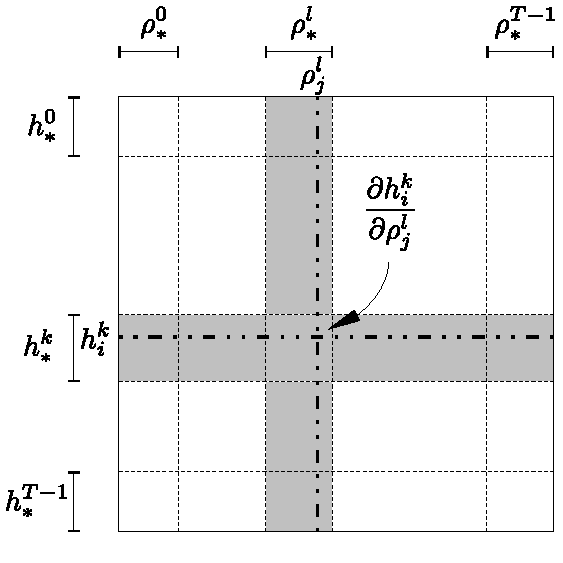
\includegraphics[width=0.45\columnwidth]{figs-gen/dstate}
												
						}\texttt{\hfill{}}\subfloat[\label{fig:sparsity-diagram}Sparsity structure of the $\Hx$ matrix.
				Besides the diagonal blocks, which are identity matrices, blocks where
				$l\neq\tind-1$ are zero.]{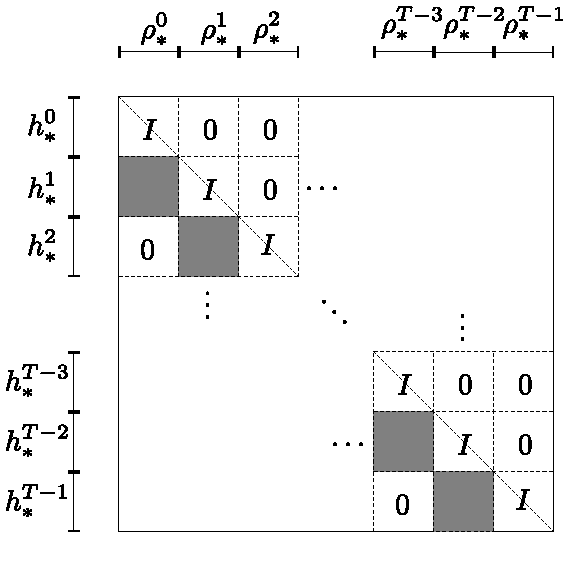
\includegraphics[width=0.45\columnwidth]{figs-gen/sparsity-two}
												
						\texttt{}
												
					}
										
					\caption{Structure of the $\Hx$ matrix.}
										
										
				\end{figure}
				Similarly for $\Hu$, we take a control parameter $\condiscrete jl\in\control$,
				and derive the expression:
								
				\begin{align}
					\pfrac{\syseq_{\link}^{\tind}}{\condiscrete jl}= & +\frac{\Delta t}{L_{i}}f'\left(\RS_{\jdown{\link}}\left(\juncstate{\jdown{\link}}{\tind-1},\junccon{\jdown{\link}}{\tind-1}\right)_{\link}\right)\pfrac{}{\condiscrete jl}\left(\RS_{\jdown{\link}}\left(\juncstate{\jdown{\link}}{\tind-1},\junccon{\jdown{\link}}{\tind-1}\right)_{\link}\right)\label{eq:dhdvfull} \\
					                                                 & -\frac{\Delta t}{L_{i}}f'\left(\RS_{\jup{\link}}\left(\juncstate{\jup{\link}}{\tind-1},\junccon{\jup{\link}}{\tind-1}\right)_{\link}\right)\pfrac{}{\condiscrete jl}\left(\RS_{\jup{\link}}\left(\juncstate{\jup{\link}}{\tind-1},\junccon{\jup{\link}}{\tind-1}\right)_{\link}\right)\nonumber                       
				\end{align}
or for the composed Godunov junction flux solver $\god_{\jn}$:
								
				\begin{equation}
					\pfrac{\syseq_{\link}^{\tind}}{\condiscrete jl}=\frac{\Delta t}{L_{i}}\left(\pfrac{}{\condiscrete jl}\left(\god_{\jdown{\link}}\left(\juncstate{\jdown{\link}}{\tind-1},\junccon{\jdown{\link}}{\tind-1}\right)\right)_{\link}-\pfrac{}{\condiscrete jl}\left(\god_{\jup{\link}}\left(\juncstate{\jup{\link}}{\tind-1},\junccon{\jup{\link}}{\tind-1}\right)\right)_{\link}\right)\label{eqdhdvgod}.
				\end{equation}
								
								
				Analyzing~\eqref{eq:dhdufull}, the only partial terms that are not
				trivial to compute are $\pfrac{}{\discrete jl}\left(\RS_{\jdown{\link}}\left(\juncstate{\jdown{\link}}{\tind-1},\junccon{\jdown{\link}}{\tind-1}\right)_{\link}\right)$
				and $\pfrac{}{\discrete jl}\left(\RS_{\jup{\link}}\left(\juncstate{\jup{\link}}{\tind-1},\junccon{\jup{\link}}{\tind-1}\right)_{\link}\right)$.
				Similarly for~\eqref{eq:dhdvfull}, the only nontrivial terms are
				$\pfrac{}{\condiscrete jl}\left(\RS_{\jdown{\link}}\left(\juncstate{\jdown{\link}}{\tind-1},\junccon{\jdown{\link}}{\tind-1}\right)_{\link}\right)$
				and $\pfrac{}{\condiscrete jl}\left(\RS_{\jup{\link}}\left(\juncstate{\jup{\link}}{\tind-1},\junccon{\jup{\link}}{\tind-1}\right)_{\link}\right)$.
				Once one obtains the solutions to these partial terms, then one can
				construct the full $\Hx$ and $\Hu$ matrices and use~\eqref{eq:adjoint}
				and~\eqref{eq:adjoint-grad} to obtain the gradient value.
								
				As these expressions are written for a general scalar conservation
				law, the only steps in computing the gradient that are specific to
				a particular conservation law and Riemann solver are computing the
				derivative of the flux function $f$ and the partial derivative terms
				just discussed. These expressions are explicitly calculated for the
				problem of optimal ramp metering in Section~(\ref{sec:Applications-to-Optimal}).
								
								
				\subsection{Complexity of solving gradient via forward method vs. adjoint method\label{sub:Complexity-of-solving}}
								
								
				\paragraph{Structure and sparsity.\label{par:Structure-and-sparsity}}
								
				We can show the lower-triangular structure and invertibility of $\Hx$
				by examining~\eqref{eq:init-ge} and~\eqref{eq:main-ge}. For $\tind\in\intrange 1{\ntime-1}$,
				we have that $\syseq_{\link}^{\tind}$ is only a function of $\discrete{\link}{\tind}$
				and of the state variables from the previous time-step $\tind-1$.
				Thus, based on our ordering scheme in Section~\ref{sec:State,-control,-and}
				of ordering variables by increasing time-step and ordering constraints
				by corresponding variable, we know for $\Hx$, diagonal terms are
				always $1$ and all upper-triangular terms must be zero (since those
				terms correspond to constraints with a dependence of \emph{future}
				values). These two conditions demonstrate both that $\Hx$ is lower-triangular
				and is also invertible due to the identity matrix block-diagonal terms.
								
				Additionally, if we consider taking partial derivatives with respect
				to the variable $\discrete jl$, then we can deduce from Equation~\eqref{eq:main-ge}
				that all partial terms will be zero except for the diagonal term,
				and those terms involving constraints at time $j+1$ with links connecting
				to the downstream and upstream junctions $\jdown j$ and $\jup j$
				respectively. To summarize, $\Hx$ matrices for systems described
				in Section~\ref{sec:State,-control,-and} will be square, invertible,
				lower-triangular and each column will have a maximum cardinality equal
				to $\degree{\state}$ in~\eqref{eq:dx}. The sparsity structure of
				$\Hx$ is depicted in Fig.~(\ref{fig:sparsity-diagram}).
								
				Using the same line of argument for maximum cardinality in $\Hx$,
				we can bound the maximum cardinality of each column of $\Hu$. Taking
				a single control variable $\condiscrete jl$, the variable can only
				appear in constraints at time-step $j+1$ that correspond to a link
				that connects to a junction $\jn$ such that $\condiscrete jl\in\junccon{\jn}{l+1}$.
				These conditions give us the expression for $\degree{\control}$ in~\eqref{eq:dv},
				or the maximum cardinality over all columns in $\Hu$.
								
				If we only consider the lower triangular form of $\Hx$, then the
				complexity of solving for the gradient using the forward system is
				$O(\left(\nlinks\ntime\right)^{2}\ncontrols\ntime)$, where the dominating
				term comes from solving~\eqref{eq:j-v}, which requires the solution
				of $\ncontrols\ntime$ separate $\nlinks\ntime\times\nlinks\ntime$
				lower-triangular systems. The lower-triangular system allows for forward
				substitution, which can be solved in $O(\left(\nlinks\ntime\right)^{2})$
				steps, giving the overall complexity $O(\left(\nlinks\ntime\right)^{2}\ncontrols\ntime)$.
				The complexity of computing the gradient via the adjoint method is
				$O(\left(\nlinks\ntime\right)^{2}+\left(\nlinks\ntime\right)\left(\ncontrols\ntime\right))$,
				which is certainly more efficient than the forward-method, as long
				as $\ncontrols\ntime>1$. The efficiency is gained by considering
				that~\eqref{eq:adjoint} only requires the solution of a single $\nlinks\ntime\times\nlinks\ntime$
				\emph{upper}-triangular system (via backward-substitution), followed
				by the multiplication of $\lambda^{T}H_{v}$, an $\nlinks\ntime\times\nlinks\ntime$
				and an $\nlinks\ntime\times\ncontrols\ntime$ matrix in~\eqref{eq:adjoint-grad},
				with a complexity of $O(\left(\nlinks\ntime\right)^{2}+\left(\nlinks\ntime\right)\left(\ncontrols\ntime\right))$.
								
				For the adjoint method, this complexity can be improved upon by considering
				the sparsity of the $\Hx$ and $\Hu$ matrices, as detailed in Section~\ref{par:Structure-and-sparsity}.
				For the backward-substitution step, each entry in the $\lambda$ vector
				is solved by \emph{at most} $\degree{\state}$ multiplications, and
				thus the complexity of solving~\eqref{eq:adjoint} is reduced to
				$O(\degree{\state}\nlinks\ntime)$. Similarly, for the matrix multiplication
				of $\lambda^{T}H_{v}$, while $\lambda$ is not necessarily sparse,
				we know that each entry in the resulting vector requires at most $\degree{\control}$
				multiplications, giving a complexity of $O(\degree{\control}\ncontrols\ntime)$. 
				\begin{prop}
					\textup{The total complexity for the adjoint method on a scalar hyperbolic
						network of PDEs is }$O(\ntime\left(\degree{\state}\nlinks+\degree{\control}\ncontrols\right))$.\end{prop}
				
